\chapter{The Compact Muon Solenoid Experiment}
\label{chap:I-3-cms}

	The Compact Muon Solenoid (CMS) \cite{1748-0221-3-08-S08004} is a multi-purpose particle detector recording the collisions provided by the LHC. It was, along with ATLAS, the first experiment officially approved for the LHC by the CERN research board in January 1997 after a long evaluation process of the letter of intent published four years earlier by the collaboration. The construction of the detector started in 2005, after the excavation works of the cavern finished, and spanned until 2008. Since then, CMS has been proficiently taking and analyzing data, and announced on July 4th 2012 the discovery of the Brout-Englert-Higgs boson, one of the most significant results of the collaboration.

  \section{Overview}

    At nominal energy and luminosity, the LHC produces around 20 proton-proton interactions per BX which results in more than 1 000 particles in the final state. In order to distinguish physical processes with great precision, CMS has to ensure good identification and reconstruction of the particles. To this end, the detector was built around four requirements, as stated in \cite{1748-0221-3-08-S08004}:
    \begin{itemize}
      \item Good muon identification and momentum resolution over a wide range of momenta and angles, good dimuon mass resolution ($ \approx $ 1\% at 100 GeV\footnote{The widely used convention that sets $ c = \hbar = 1 $ is used through out this work in order to express energies and masses in electronvolts. A factor of $c^{-1}$ and $c^{-2}$ should respectively be applied to these numbers in order to obtain the values in the international unit system.}), and the ability to determine unambiguously the charge of muons with momentum < 1 TeV;
      \item Good charged-particle momentum resolution and reconstruction efficiency in the inner tracker. Efficient triggering and offline tagging of $ \tau $'s and b-jets, requiring pixel detectors close to the interaction region;
      \item Good electromagnetic energy resolution, good diphoton and dielectron mass resolution ($ \approx $ 1\% at 100 GeV), wide geometric coverage, $ \pi^0 $ rejection, and efficient photon and lepton isolation at high luminosities;
      \item Good missing-transverse-energy and dijet-mass resolution, requiring hadron calorimeters with a large hermetic geometric coverage and with fine lateral segmentation. \\
    \end{itemize}

    \begin{figure}[h!]
      \centering
      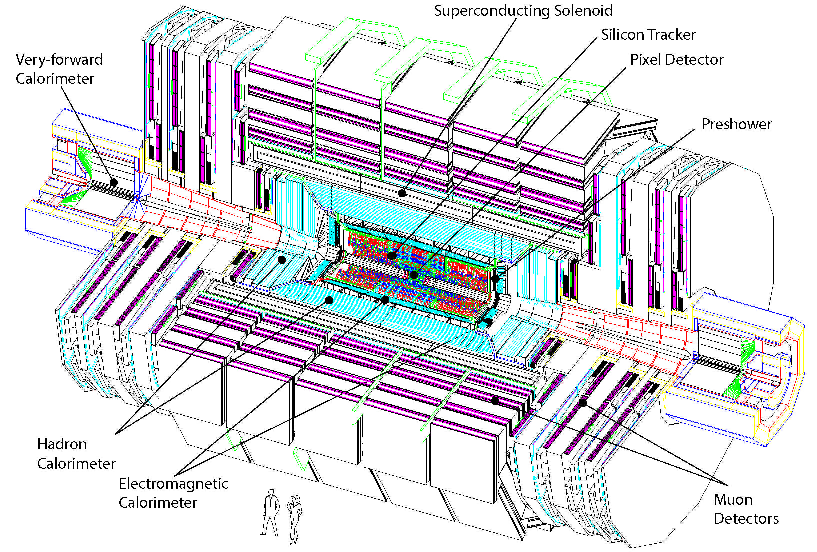
\includegraphics[width=0.9\textwidth]{img/I-3-cms/cms.pdf}
      \caption{The Compact Muon Solenoid detector and its subsystems installed at LHC \cite{1748-0221-3-08-S08004}.}
      \label{fig:I-3-cms-global-view}
    \end{figure}

    These requirements are met through the subdivision of CMS in various detection systems each specialized in the reconstruction of a given type of particles. The overall layout of CMS, shown in Figure \ref{fig:I-3-cms-global-view}, is divided into the barrel and the two endcaps, regions where the detectors are respectively placed in parallel and perpendicularly to the beam pipe. At the center of the detector, within a radius of 1.25 m around the beam pipe, lies the inner tracking system. Composed of three layers of silicon pixels and ten layers of silicon strips detectors, it is designed to detect the passage of any charged particle with a spatial resolution on the order of 50 $\mu$m. Surrounding the tracking system are the electromagnetic and hadron calorimeters which respectively measure the energy of electrons and photons, and hadrons through the annihilation of the latter within the detectors. These systems are placed inside a superconducting solenoid magnet which produces a strong 3.8 T field that bends charged particles and allows for precise momentum measurements. The obtained resolution on the transverse momentum is so that $\frac{\Delta p_T}{p_T} \approx 1\% $ for 100 GeV muons in the barrel. Outside of the magnet, three different technologies of muon detectors are placed on large iron yokes. \\

    The coordinate system used in CMS has its origin at the nominal interaction point of the beams, the y-axis pointing upwards, the x-axis pointing toward the center of the LHC, and the z-axis directed along the beam direction. The polar coordinates (r, $ \phi $) are defined in the x-y transverse plane and the widely used pseudorapidity $ \eta $ is taken to be
    \begin{equation}
      \eta = - \ln\left( \tan\left( \frac{\theta}{2} \right) \right) ,
    \end{equation}
    where $ \theta $ is the azimuthal angle between the z-axis and the transverse plane.

  \section{The Inner Tracking System}

    The inner tracking system of CMS provides a spatial resolution on the order of 50 $\mu$m with a detection efficiency above 99\% for the passage of charged particles. The proximity of the detectors to the beam pipe yields a high particle density of up to 10$^8$ particles per cm$^2$ at a radius of 4 cm. This justifies the need for a high granularity and fast response time to unambiguously assign particles to the correct collision. This is achieved through a density of up to 4 000 channels per cm$^2$  and a time resolution of 6 ns. However, these features come with an elevated power consumption of a few microwatts per channel which in turn requires a cooling infrastructure to maintain the tracker at a temperature of -20 $^o$C. In order to minimize the material budget of the tracker, a compromise was found to use two technologies: silicon pixels close to the beam pipe to provide a high granularity, and silicon strips further away to minimize the material budget. \\

    The layout of the detectors is shown in Figure \ref{fig:I-3-tracker}. The silicon pixels (PIXEL) are installed on three cylindrical layers in the barrel and two disks in each endcap. These detectors cover an area between radii of 4.4 cm and 10.2 cm and a pseudorapidity $|\eta|$ < 2.5. The silicon strips (TIB, TID, TOB, and TEC) occupy a radial region between 20 cm and 116 cm and are divided in different sectors with a total of 10 layers in the barrel and 12 disks in each endcap. The segmentation into sectors corresponds to the various strip geometries and arrangement. \\

    \begin{figure}[h!]
      \centering
      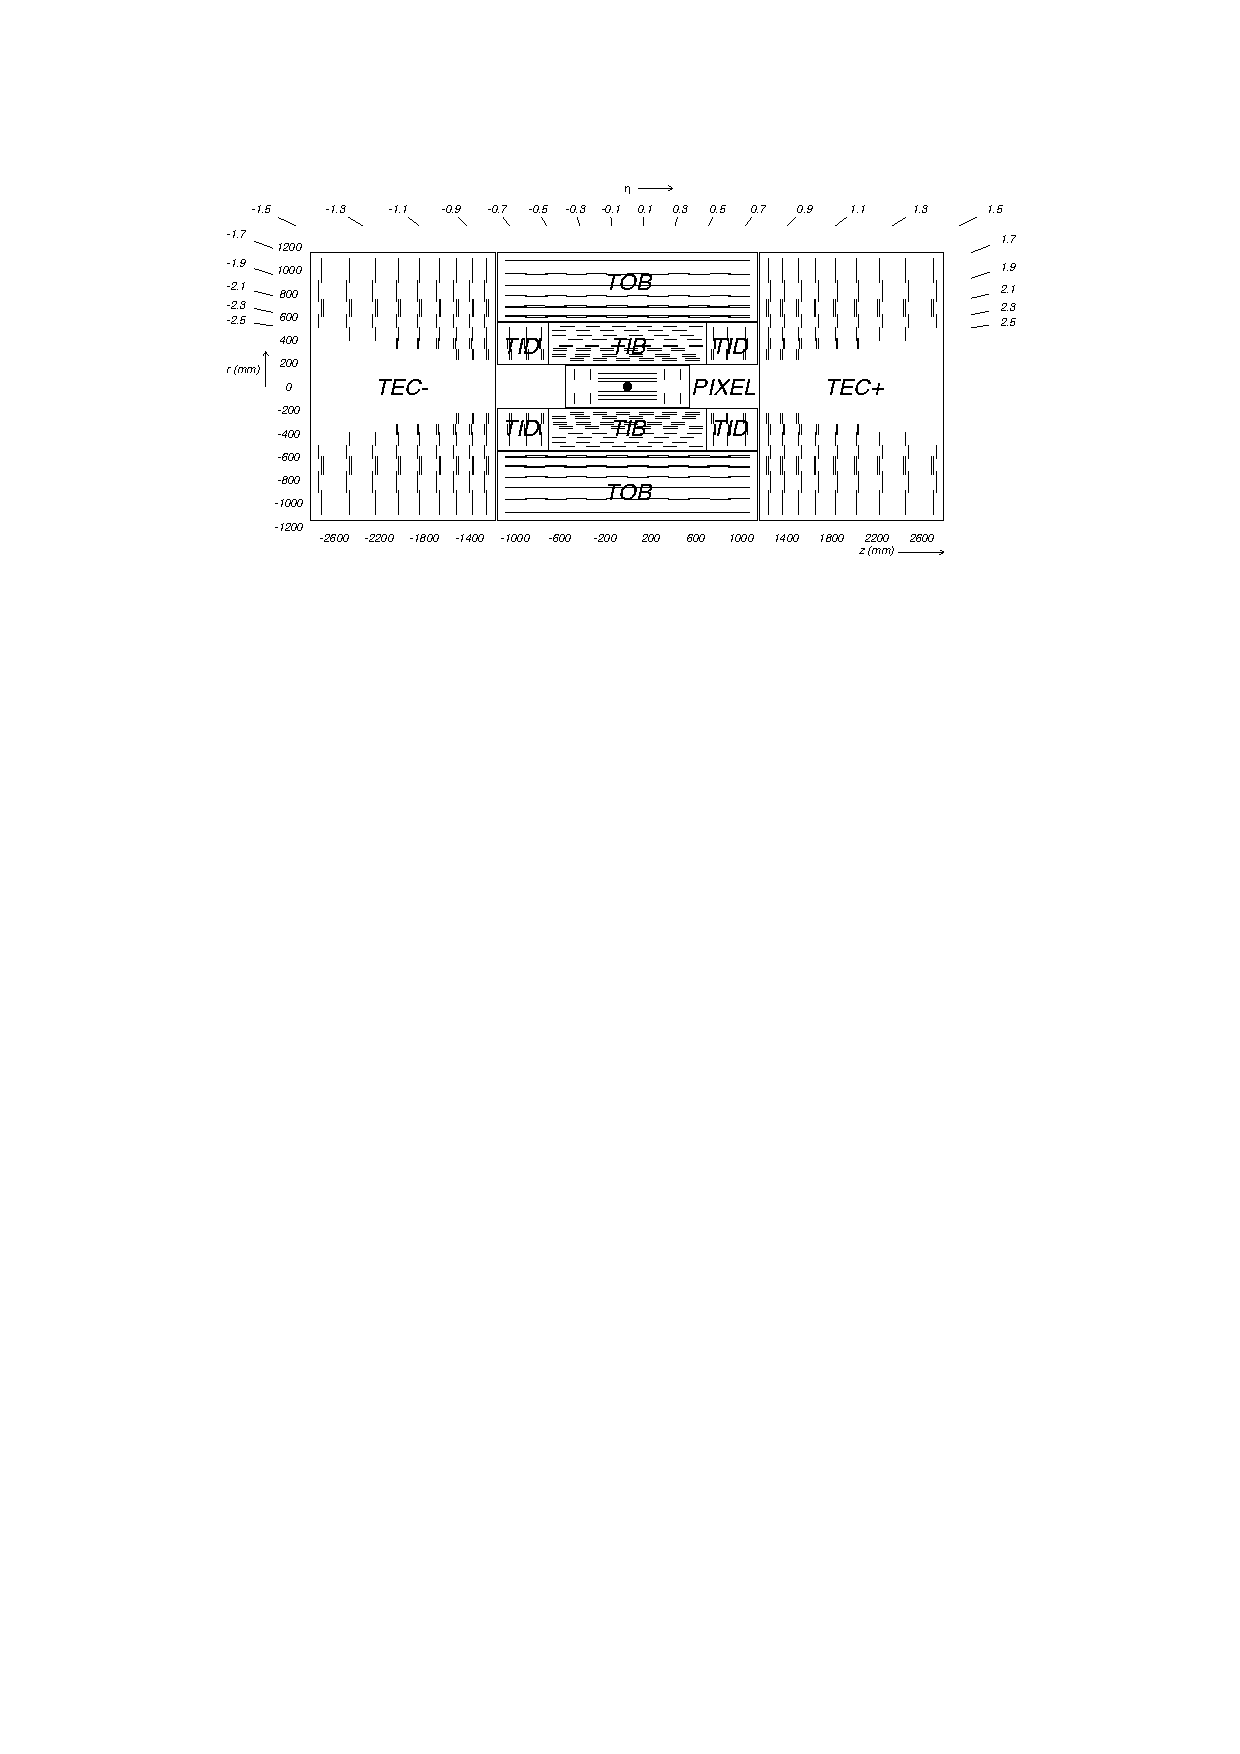
\includegraphics[width=0.86\textwidth]{img/I-3-cms/tracker.pdf}
      \caption{Disposition of the silicon pixels (PIXEL) and strips (TIB, TID, TOB, and TEC) modules inside the tracker of CMS \cite{1748-0221-3-08-S08004}.}
      \label{fig:I-3-tracker}
    \end{figure}

    The barrel pixel tracker contains 768 modules for a total of 48 million pixels. The disks of the endcaps are divided into 24 segments each composed of 7 modules which yield a total number of 672 modules with 18 million pixels for both endcaps. Each pixel is 150 $\mu$m $\times$ 100 $\mu$m in size with a thickness of 260 $\mu$m to 300 $\mu$m resulting in a single point hit resolution of 15 $\mu$m to 20 $\mu$m. \\

    The silicon strip tracker is divided into three subsystems. The Tracker Inner Barrel and Disks (TIB and TID) are composed of 4 layers in the barrel and 3 disks in each endcap, covering a region up to a radius of 55 cm. The strips are 320 $\mu$m thick and run parallel to the beam pipe in the barrel and radially in the disks. The strip pitch is of 80 $\mu$m in the two first layers of the TIB and 120 $\mu$m in the two next ones, resulting in a spatial resolution of respectively 23 $\mu$m and 35 $\mu$m. In the TID, the pitch varies between 100 $\mu$m and 141 $\mu$m. Surrounding the TIB and TID is the Tracker Outer Barrel (TOB) composed of 6 barrel layers of 500 $\mu$m thick strips. It provides a resolution of 53 $\mu$m for the first four layers and 35 $\mu$m for the two last ones. Closing the TOB on both sides are the Tracker EndCaps (TEC) which each holds 9 disks. Additionally, the modules of the two inner layers of the TIB and TOB, the two inner rings of the TID and TEC, and the fifth ring of the TEC are equipped with a second strip detector mounted back-to-back with a stereo angle of 100 mrad and provides a measurement of the second coordinate. \\

    The detection efficiency above 99\% and spatial resolution below 53 $\mu$m of the tracker allows it to achieve a track reconstruction efficiency above 98\% in the $|\eta|$ < 2 region (a dip in efficiency is present at $\eta$ = 0 due to the gap between modules) with a transverse momentum resolution better than 3\% for 100 GeV muons. Figure \ref{fig:I-3-tracker-eff} depicts the track reconstruction efficiency (left) and transverse momentum resolution (right) of the tracker for single muons with transverse momenta of 1, 10 and 100 GeV. \\

    \begin{figure}[h!]
      \centering
      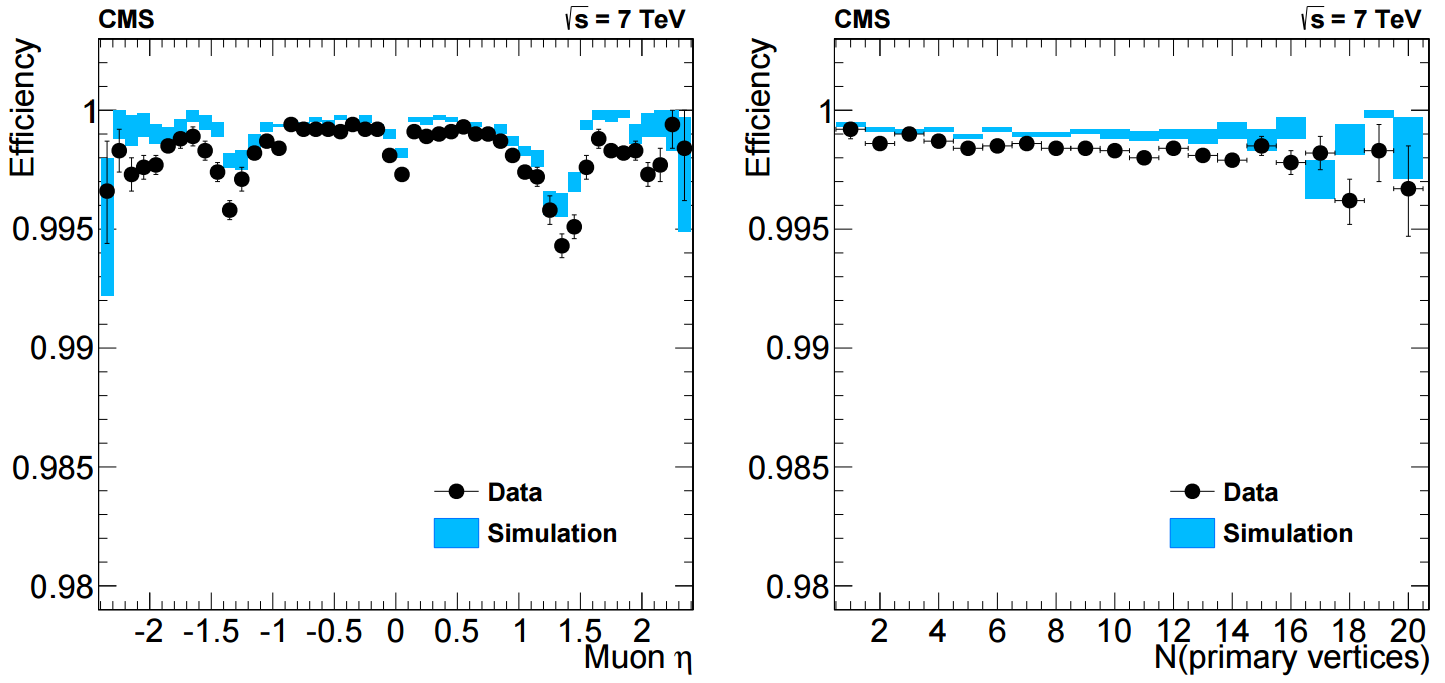
\includegraphics[width=\textwidth]{img/I-3-cms/tracker_efficiency.png}
      \caption{Track reconstruction efficiency (left) and transverse momentum resolution (right) of the tracker for single muons with transverse momenta of 1, 10 and 100 GeV \cite{1748-0221-3-08-S08004}.}
      \label{fig:I-3-tracker-eff}
    \end{figure}

    The resulting material budget of the tracker is shown in Figure \ref{fig:I-3-tracker-material} in which it is expressed in terms of radiation length $X_0$ on the left and hadronic interaction length $\lambda_I$ on the right. From the quantity of material in the tracker, 70\% of the photons materialize into an e$^+$/e$^-$ pair and 5\% of 5 GeV pions interact within its volume.

    \begin{figure}[h!]
      \centering
      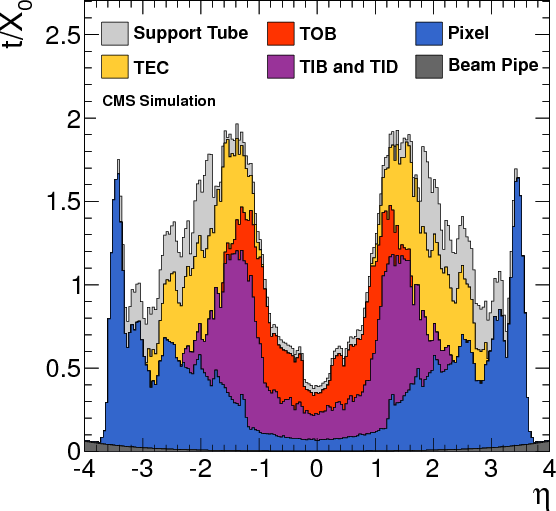
\includegraphics[width=0.49\textwidth]{img/I-3-cms/tracker_budget_e.png}
      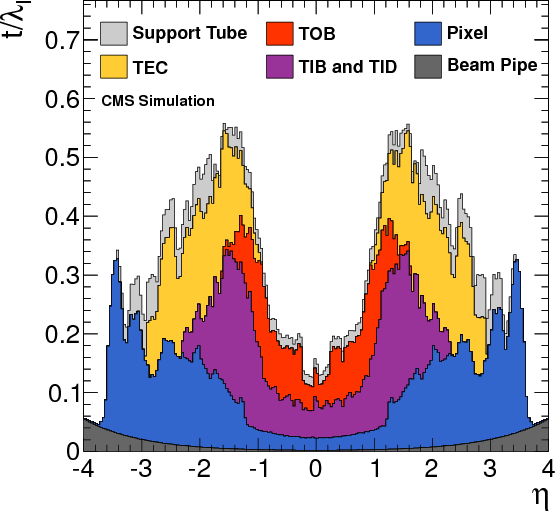
\includegraphics[width=0.49\textwidth]{img/I-3-cms/tracker_budget_h.png}
      \caption{Material budget of the tracker expressed in terms of radiation length $X_0$ on the left and hadronic interaction length $\lambda_I$ on the right \cite{1748-0221-3-08-S08004}.}
      \label{fig:I-3-tracker-material}
    \end{figure}

  \section{The Electromagnetic Calorimeter}

    The Electromagnetic Calorimeter (ECAL) of CMS has been designed to provide an energy resolution for electrons and photons of the order of 1\% for 100 GeV. It is composed of lead tungsten (PbWO$_4$) crystals that act as homogeneous calorimeters: they both initiate the particle cascades and provide the proportional response to the energy deposition. The barrel counts 61 200 crystals closed by 7 324 crystals in each endcap. Additionally, a silicon preshower detector is installed in front of the crystals in the endcaps to improve the detection of collimated particles. \\

    The structure of the ECAL is shown in Figure \ref{fig:I-3-ecal}. In the barrel, the ECAL covers a pseudorapidity range $ | \eta | $ < 1.479 and is divided in 360 sections in $ \phi $ and 170 in $ \eta $. The cross section of the crystals varies between 22 mm $ \times $ 22 mm to 26 mm $ \times $ 26 mm for a length of 230 mm corresponding to 25.8 radiation lengths. An alveolar structure maintains crystals together in submodules which are grouped into modules of 400 to 500 crystals further assembled in supermodules containing 1700 crystals in total. In the endcaps, modules cover a pseudorapidity of 1.479 < $ | \eta | $ < 3.0 with each crystal having a front cross-section of 28.62 mm $ \times $ 28.62 mm and a length of 220 mm. These are grouped in units of 5 $ \times $ 5 crystals called supercrystals further inserted in one of the two \emph{Dees} that compose an endcap and maintains the ECAL in place. The preshower uses a lead radiators to initiate the avalanche that will be detected by silicon strips to measure the deposited energy and the avalanche profile. Each sensitive module has an active area of 61 mm $\times$ 61 mm divided among 32 strips. The preshower is installed in the 1.653 < $ | \eta | $ < 2.6 pseudorapidity region. \\

    \begin{figure}[h!]
      \centering
      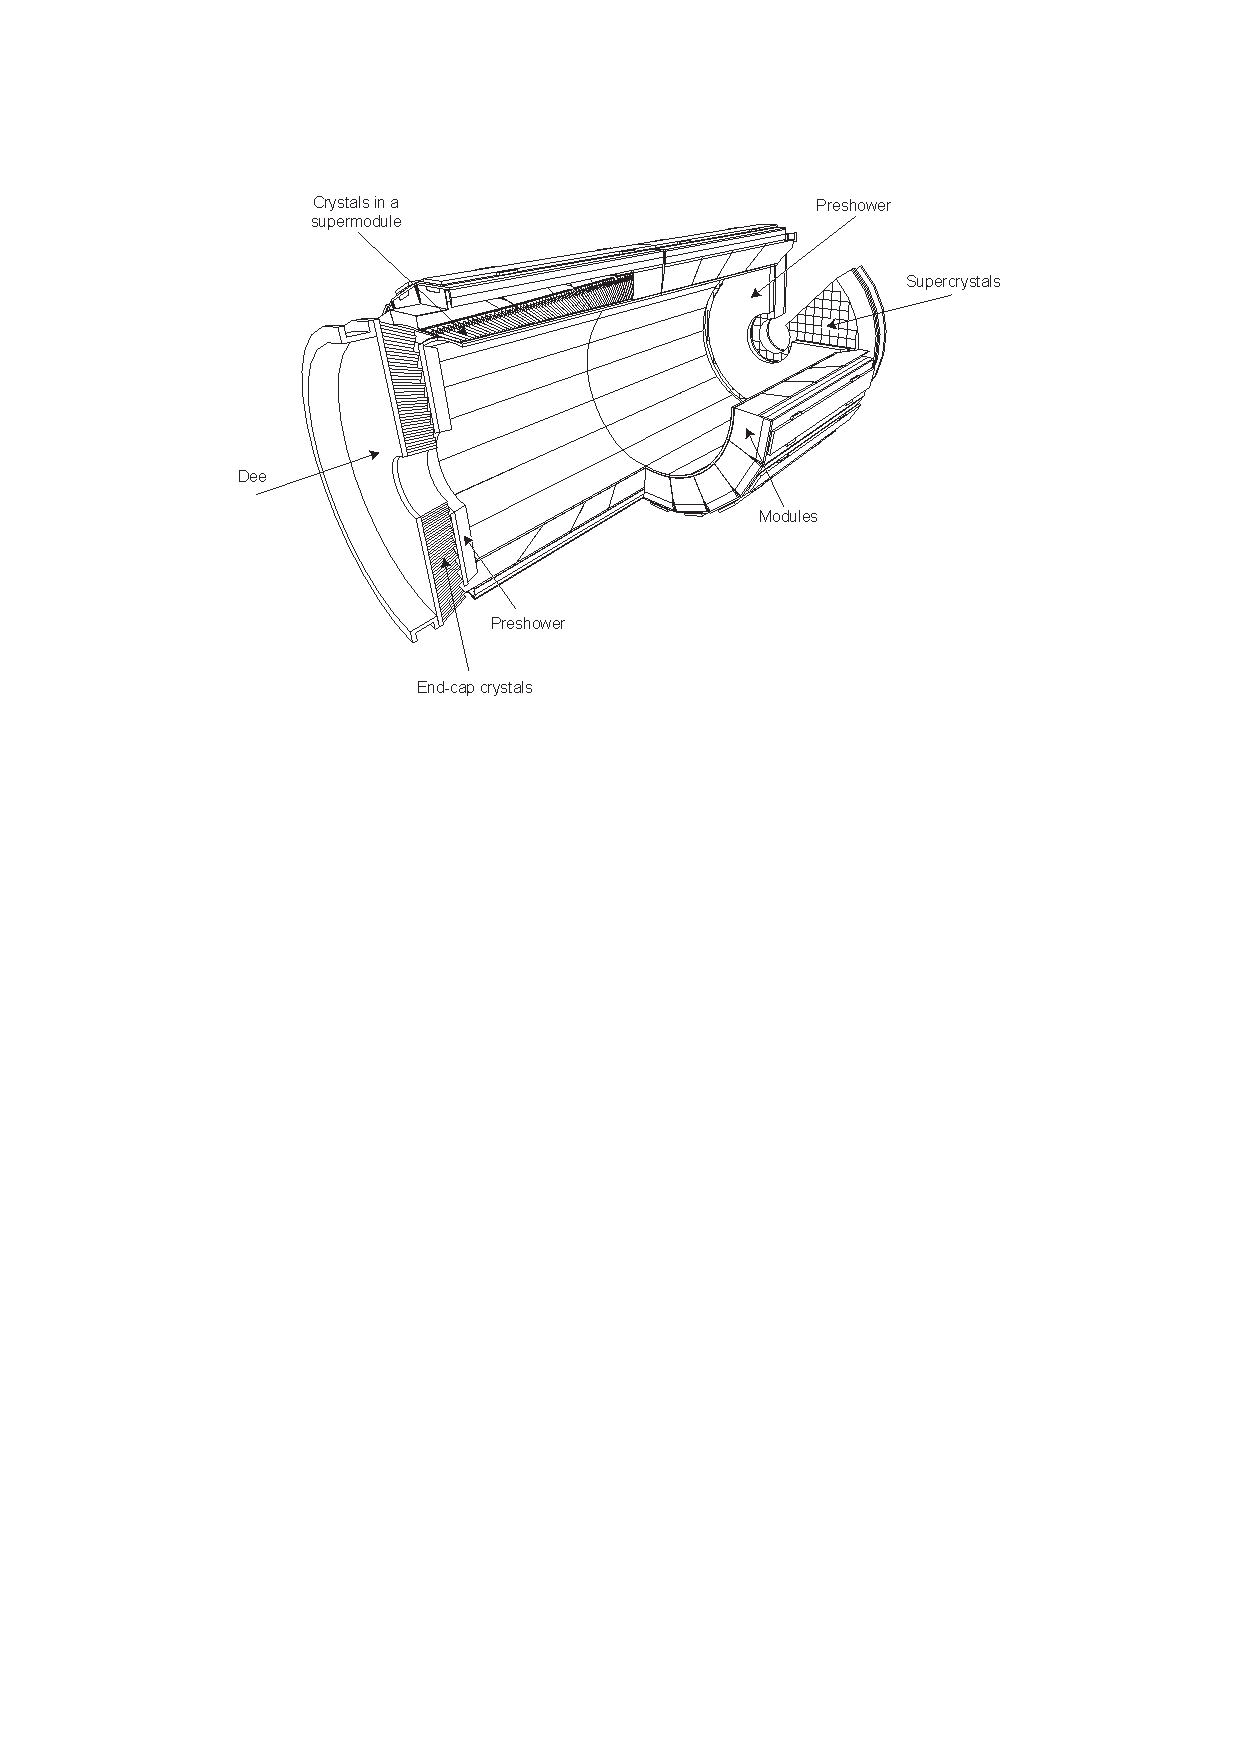
\includegraphics[width=0.7\textwidth]{img/I-3-cms/ecal.pdf}
      \caption{Layout of the ECAL showing the disposition of the crystals, modules, supermodules, and preshower \cite{1748-0221-3-08-S08004}.}
      \label{fig:I-3-ecal}
    \end{figure}

    The energy resolution of the ECAL for particles with energy bellow 500 GeV is parametrized by the following equation:
    \begin{equation}
      \left( \frac{\sigma}{E} \right)^2 = \left( \frac{S}{\sqrt{E}} \right)^2 + \left( \frac{N}{E} \right)^2 + C^2
    \end{equation}
    where $ S $ is the stochastic term, $ N $ the noise term, and $ C $ the constant term. The main contributions to the stochastic term are related to fluctuations in the lateral shower containment, photostatistics contributions, and fluctuations in the energy deposition inside the preshower radiators compared to what is measured by the silicon detector. The noise term includes noise from the electronics, the digitization, and pile-up. Finally, the constant term accounts for non-uniformities in the crystals, calibration errors, and leakage of energy from the back of the crystals. From test beams, the values of $ S $, $ N $, and $ E $, were found to be so that: \\
    \begin{equation}
      \left( \frac{\sigma}{E} \right)^2 = \left( \frac{2.8\%}{\sqrt{E}} \right)^2 + \left( \frac{0.12}{E} \right)^2 + (0.30\%)^2
    \end{equation}

  \section{The Hadron Calorimeter}

    The Hadron Calorimeter (HCAL) provides a measurement of the energy of the hadronic jets and enables the computation of the missing energy. It is divided into a barrel region (HB), two endcaps regions (HE), and an outer calorimeter (HO) placed right outside the magnet as represented in Figure \ref{fig:I-3-hcal}. The HB sits between the ECAL and the magnet at radii of 1.77 m and 2.95 m respectively, which limits the amount of material and thus absorption lengths that can be used, justifying the need for the HO to catch the trail of the cascades. An additional forward calorimeter (HF) is placed in the very forward region of CMS to analyze particles that are produced or scattered at $ \eta $ > 3. \\

    \begin{figure}[h!]
      \centering
      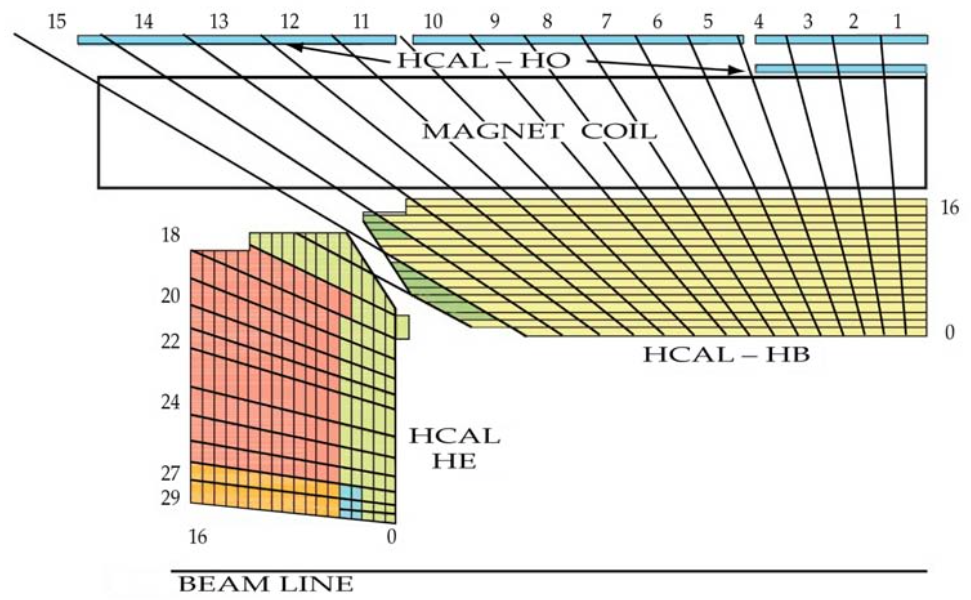
\includegraphics[width=\textwidth]{img/I-3-cms/hcal.png}
      \caption{Longitudinal view of the HCAL showing the disposition of the barrel, endcaps, and outer calorimeters \cite{1748-0221-3-08-S08004}.}
      \label{fig:I-3-hcal}
    \end{figure}

    The HB uses a sampling calorimeter design that consists of a succession of metal sheets positioned parallel to the beam that act as absorber, and plastic scintillators to measure the energy deposition. The absorber is made of a 40-mm-thick front steel panel, followed by eight 50.5-mm-thick brass sheets, six 56.5-mm-thick brass panels, and a 75-mm-thick steel back plate for a total minimum of 5.82 interaction lengths. The scintillators are designed out of 3.7-mm-thick Kuraray SCSN81 plastic and placed after each layer of metal. An additional layer of 9-mm-thick Bicron BC408 is placed in front of the first steel panel in order to sample hadronic showers that might have formed in the ECAL. The scintillator is divided into 16 $ \eta $ and 72 $ \phi $ sectors resulting in a segmentation of $ \Delta \eta \times \Delta \phi $ = 0.087 $ \times $ 0.087. The HE uses 79-mm-thick brass plates spaced by 9 mm gaps in which the plastic Bicron BC408 scintillators are inserted. The segmentation of the HE results in a granularity similar to the HB for $ | \eta | $ < 1.6 and of $ \Delta \eta \times \Delta \phi $ = 0.17 $ \times $ 0.17 for $ | \eta | $ $ \le $ 1.6. In the $ | \eta | $ < 1.3 region, hadron showers are not entirely contained in the HB and HE thus justifying the installation of the HO outside of the magnet to catch the trail of the cascades. This has a significant impact on high energy cascades and to measure the missing energy of an event, i.e. the energy carried by non-interacting particles. The HO has a minimum thickness of 1.4 interaction lengths and is segmented in 5 rings further divided into segments. Each segment has a granularity similar to the HB of 0.087 $ \times $ 0.087 in $ \Delta \eta \times \Delta \phi $. Limited by the muon system, the HO has been allocated 40 mm of space, from which 16 mm are used for the scintillators and the rest is filled with support material. \\

    The energy resolution of the HCAL can be expressed in the same manner as the ECAL, breaking down the result into a stochastic term and a constant term. The obtained resolutions \cite{Baiatian:1049929} are
    \begin{equation}
      \left( \frac{\sigma}{E} \right)^2 = \left( \frac{120\%}{\sqrt{E}} \right)^2 + (9.5\%)^2
    \end{equation}
    for the HB and HE combined, and
    \begin{equation}
      \left( \frac{\sigma}{E} \right)^2 = \left( \frac{280\%}{\sqrt{E}} \right)^2 + (11\%)^2
    \end{equation}
    for the HO.

  \section{The Superconducting Magnet}

    The superconducting magnet of CMS measures 6 m of diameter for 12.5 m in length and has been designed to generate a 4 T magnetic field. The return of the magnetic field lines is done through the steel yokes that support the muon chambers of CMS as represented in Figure  \ref{fig:I-3-cms-magnet} in which the amplitude of the magnetic field has been simulated. The magnet is composed of four layers of winded NbTi conductor which offers very low resistance to the nominal 19.14 kA current that is required to generate the field. To reach the superconducting state of the magnet, the latter needs to be cooled down to 1.8 K using liquid Helium. The magnetic field thereby created bends charged particles according to their transverse momentum in the x-y plane
    \begin{equation}
      R = \frac{p_T}{0.3 B} ,
    \end{equation}
    where $ R $ is the curvature radius of the trajectory in the transverse plane, $ p_T $ is the transverse momentum of the particle expressed in GeV, and $ B $ is the intensity of the magnetic field in T.

    \begin{figure}[h!]
      \centering
      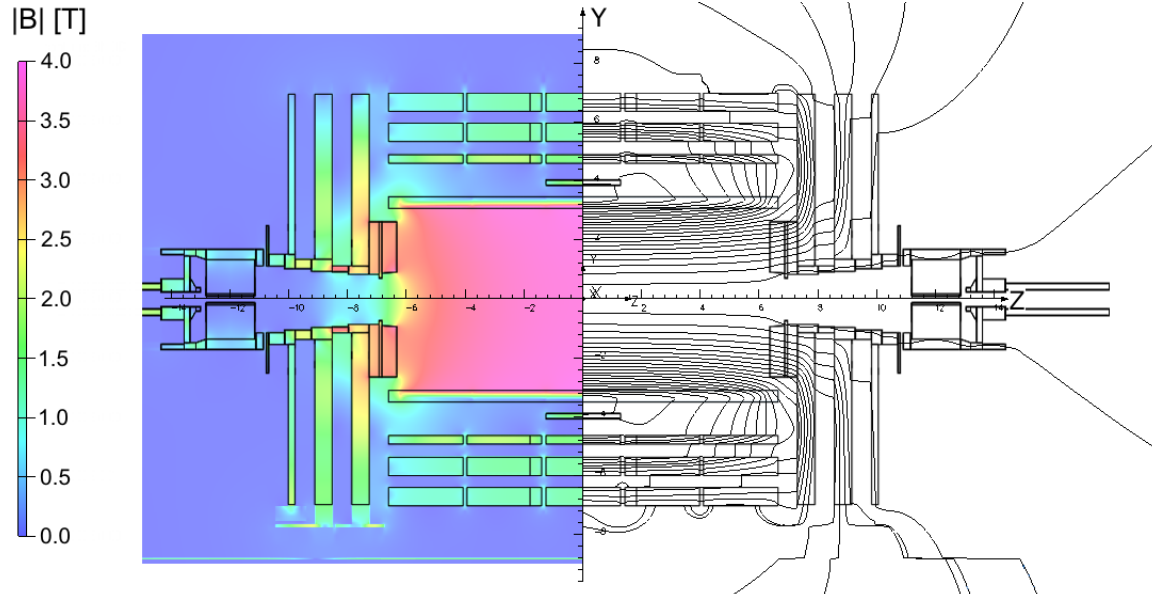
\includegraphics[width=0.8\textwidth]{img/I-3-cms/magnet.png}
      \caption{Representation of the amplitude of the magnetic field and the field lines predicted on a longitudinal section of the CMS detector using simulations \cite{Chatrchyan:2009si}.}
      \label{fig:I-3-cms-magnet}
    \end{figure}

  \section{The Muon System}

    Muons are a recognizable signature from the high background noise produced by the large number of proton-proton interactions. Moreover, they are present in many final states that characterize interesting processes from the Standard Model and beyond. Therefore, providing identification capabilities better than 98\% is essential. CMS is equipped with three different muon detectors that together form the muon spectrometer: Drift Tubes (DTs), Cathode Strip Chambers (CSCs), and Resistive Plate Chambers (RPCs). DTs and CSCs are respectively placed in the barrel and the endcaps while RPCs are installed in both regions, adding redundancy to the system by providing additional measurement points. Figure \ref{fig:I-3-muons} represents a quadrant of CMS highlighting the placement of the various technologies inside the detector. \\

    \begin{figure}[h!]
      \centering
      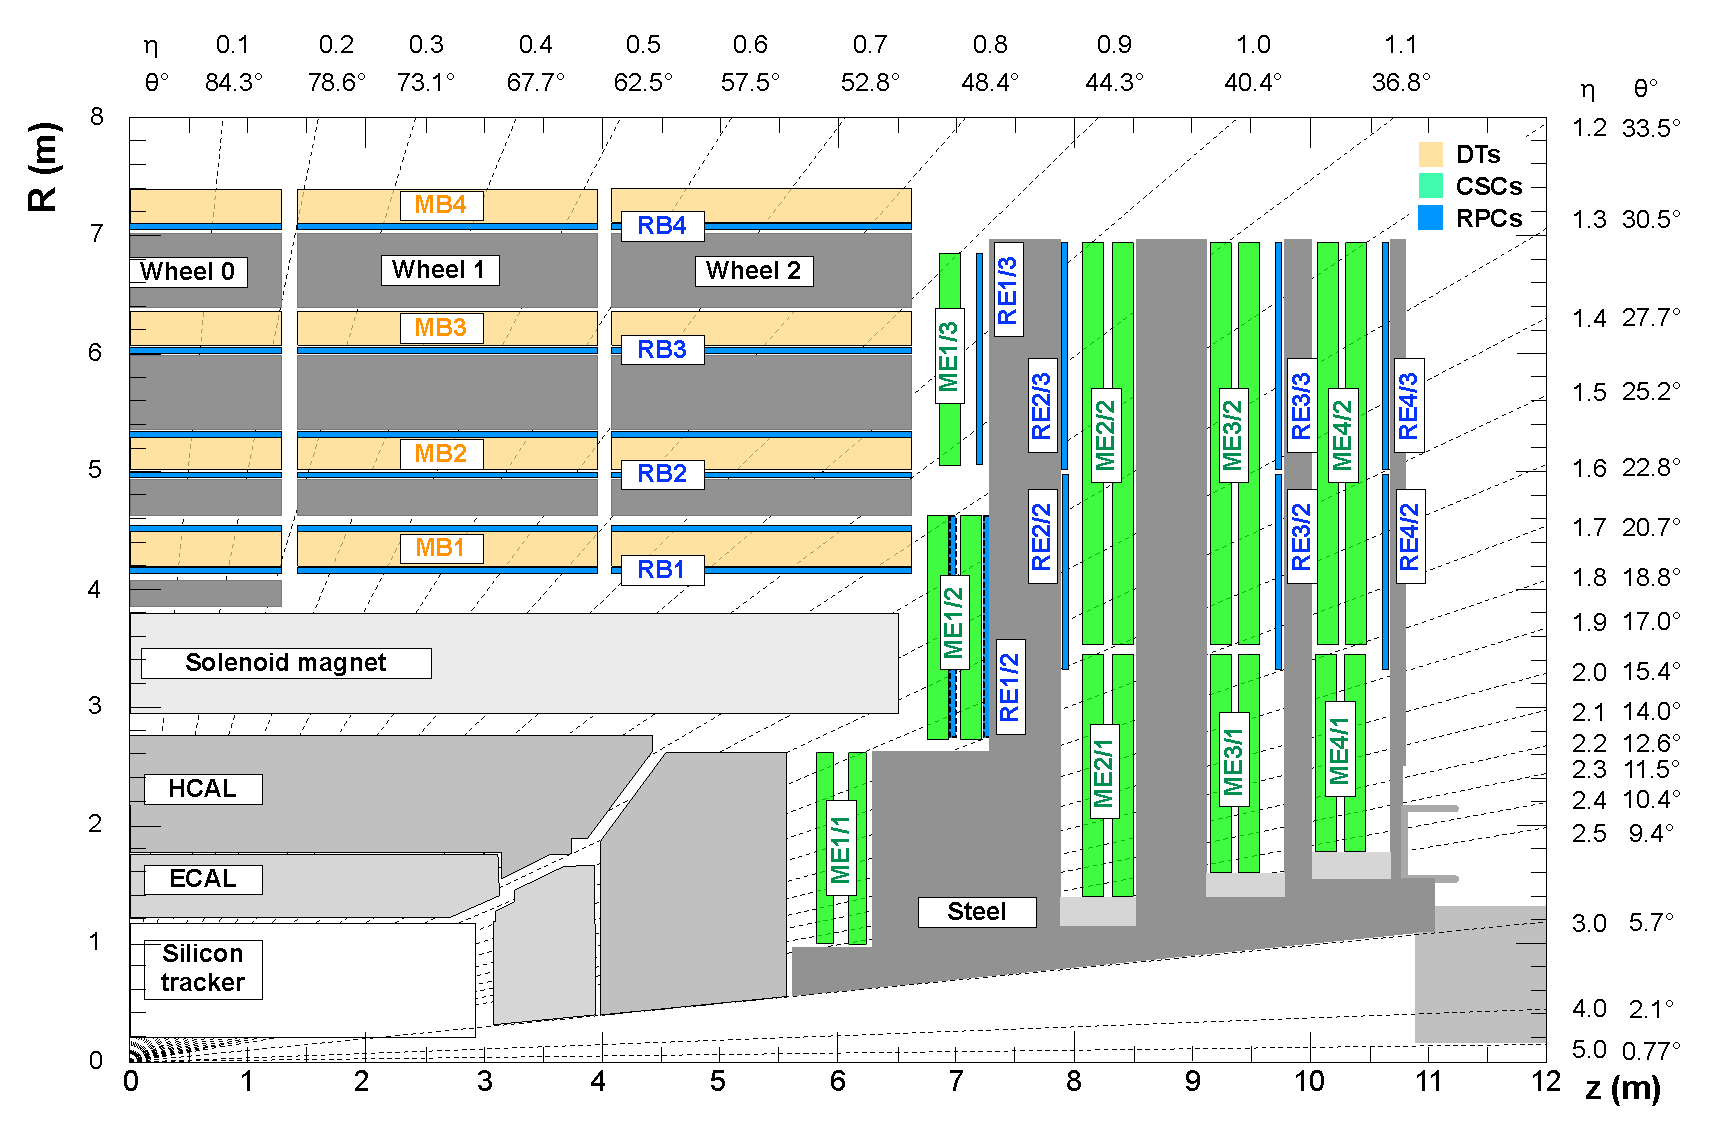
\includegraphics[width=\textwidth]{img/I-3-cms/muons.pdf}
      \caption{Layout of the muon spectrometer of CMS depicting the three gaseous detectors in use: Drift Tubes (DTs) in orange labeled MBx, Cathode Strip Chambers (CSCs) in green labeled MEx/y, and Resistive Plate Chambers (RPCs) in blue labeled RBx and REx/y \cite{1748-0221-3-08-S08004}.}
      \label{fig:I-3-muons}
    \end{figure}

    In the barrel, four cylindrical layers of DTs, numbered MB1 to MB4, cover a pseudorapidity range of $ | \eta | $ < 1.2. The first three layers each contain twelve chambers: eight to measure the r-$\phi$ bending angle and four to measure the z direction. The fourth station solely tracks the r-$\phi$ parameter using eight chambers. \\

    In the endcaps, the CSCs cover a region of 0.9 < $ | \eta | $ < 2.4 and are spread over four disks where detectors are placed perpendicularly to the beam pipe. Each disk is further divided into two or three rings numbered MEx/y, where x is the disk number and y is the ring number. CSCs measure both the r-$\phi$ and the $ \eta $ coordinates using respectively cathode strips that run radially and anode wires that run perpendicular to the strips. Each module is composed of 6 layers of CSCs which provide precise background noise rejection and tracking. \\

    Additionally, RPCs are installed along with the DTs and CSCs label RBx and REx/y respectively. In the barrel, two stations of RPCs are installed in RB1 and RB2 while only one station is instrumented in RB3 and RB4. In the endcaps, one module of RPCs equips each of the stations except for the first ring of each disk which has been left empty. This is due to the high rate of particles in the region close to the beam pipe, up to 50 kHz cm$^{-2}$, which is not supported by the RPCs.

    \subsection{Drift Tubes}

      The barrel muon spectrometer consists in 4 cylindrical layers of DT modules: the inner three contain 60 chambers and the outer has 70 for a total of 172 000 sensitive wires. The smallest unit composing the DTs is the drift cell: a 2.4 m long by 42 mm wide tube in which a wire is stretched over the whole length as depicted in Figure \ref{fig:I-3-dt}. Filled with a gas mixture of ArCO$_2$, they provide a measurement of the point of impact of the particle in the direction perpendicular to the wire using the ionization of the gas amplified through the applied high voltage. The small flux of particles in the barrel region of CMS, of the order of 2 Hz cm$^{-2}$, enables the use of these long chambers which limits the number of active channels and thus cost while still providing a spatial resolution in the 80-120 $\mu$m range. Multiple drift cells are combined into layers and four layers are further staggered by half a cell width in order to eliminate dead space and form a super layer (SL). SLs vary in size between 1.9 m in MB1 and 4.1 m in MB4. Each chamber contains two SLs that measure the r-$\phi$ bending angle and one SL that provides a measurement in the z direction. MB4, the fourth station, however does not include the SLs in the z direction. The resolution of a station is on the order of 100 $\mu$m on the position and 1 mrad on the direction of the particle. \\

      \begin{figure}[h!]
        \centering
        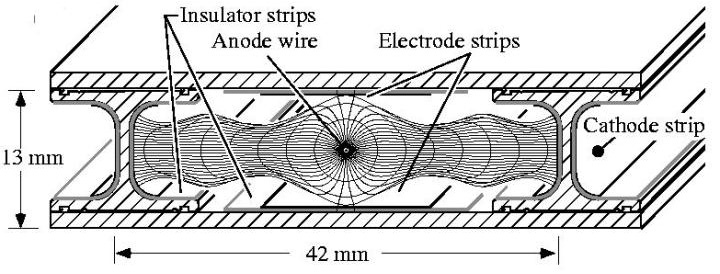
\includegraphics[width=0.8\textwidth]{img/I-3-cms/dt.jpg}
        \caption{Sketch of the drift cells highlighting the electric field lines converging towards the anode wire \cite{1748-0221-3-08-S08004}.}
        \label{fig:I-3-dt}
      \end{figure}

  	\subsection{Cathode Strip Chambers}

      The CSCs are multiwire proportional chambers made of 6 anode wire planes interleaved among 7 cathode strip panels. The largest chambers measure 3.4 m $ \times $ 1.5 m and are installed in the ME2/2, ME3/2, and ME4/2 stations while smaller chambers are mounted in the other stations limited by the steel yoke layout. Taking advantage of the multiple detection layers of the chambers, CSCs can provide a detection efficiency better than 99\%, 75 $\mu$m resolution in the r-$\phi$ coordinate for ME1/1 and ME1/2 and about 150 $\mu$m elsewhere, and a BX assignment efficiency of 99\%. \\

      The structure of the CSCs is shown in Figure \ref{fig:I-3-csc}. Seven 16.2-mm-thick trapezoidal panels made of 12.7-mm-thick polycarbonate core with two 1.6 mm FR4 skins glued on each side are assembled in order to form one chamber. FR4 is a material used to create printed circuit board. On six of the planes, 36 $\mu$m thick copper strips are milled on one side to form the cathode planes. Gap bars are glued to the planes in order to form six gaps of 9.5 mm once the planes are stacked together. About 1000 anode wires are winded around three of the panels in order to form the anode planes. The 50-$\mu$m-thick gold-plated tungsten wires are separated by 3.2 mm and elevated by 4.75 mm with respect to the plane in order to sit in the middle of the gap.

      \begin{figure}[h!]
        \centering
        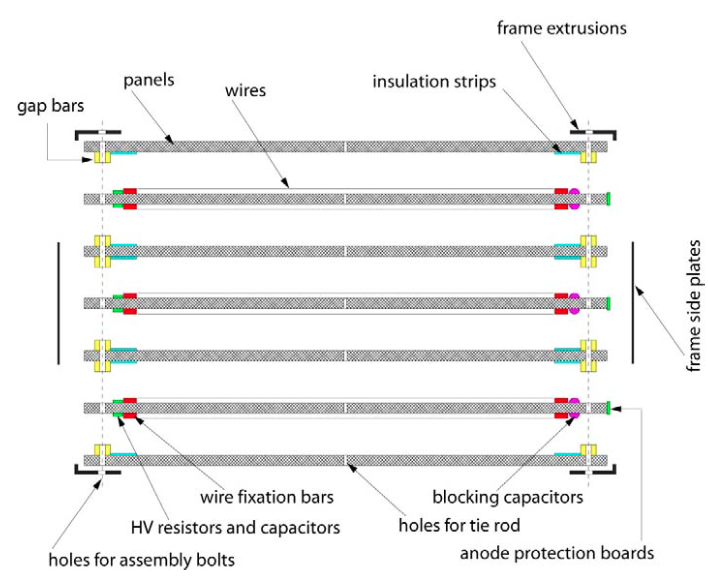
\includegraphics[width=0.8\textwidth]{img/I-3-cms/csc.png}
        \caption{Schematic view of a CSC detailing the different layers that compose it \cite{1748-0221-3-08-S08004}.}
        \label{fig:I-3-csc}
      \end{figure}

  	\subsection{Resistive Plate Chambers}

      RPCs are used for their excellent time resolution of less than 3 ns which allows them to unambiguously assign events to their corresponding BX while also providing a spatial resolution of the order of the centimeter. Each module consists in two gas filled gaps with a common read-out strip layer in the middle as depicted in Figure \ref{fig:I-3-rpc}. On each side of the gaps, an insulating backelite panel is covered with a conducting graphite layer on which a high voltage is applied. This layout allows to operate each gap at a lower high voltage and reduce the read-out time required, thus improving the time resolution. \\

      \begin{figure}[h!]
        \centering
        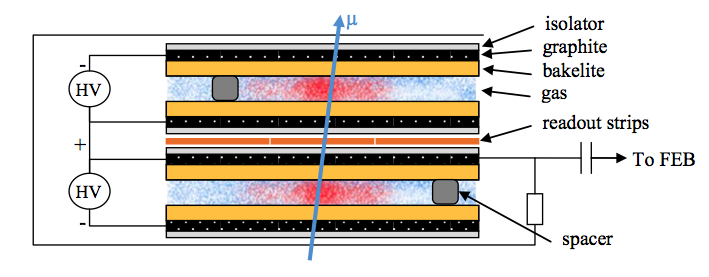
\includegraphics[width=0.7\textwidth]{img/I-3-cms/rpc.png}
        \caption{Diagram of the RPCs double gap layout \cite{1748-0221-3-08-S08004}.}
        \label{fig:I-3-rpc}
      \end{figure}

      In the barrel, RB1 and RB2 each include two RPCs placed on both sides of the DTs. RB3 and RB4 only use one RPC mounted in front of the DTs. In total, 480 chambers are installed, each with a length varying between 2.455 m long and a width between 1.5 m and 2.08 m. In the endcaps, RPCs cover a pseudorapidity range of $ | \eta | $ < 1.6 divided into two rings. Chambers are trapezoidal and cover 20$^o$ in $ \phi $ for the inner ring and 10$^o$ for the outer ring. This setup leaves an empty region between 1.6 < $ | \eta | $ < 2.45 where CSCs are the only detectors providing measurements.

  \section{The Trigger System}

    Every 25 ns approximately 20 proton-proton interactions resulting from the collisions of the LHC occur, yielding more than 1 000 particles in the final state. Each collision generates more than one MB of data which makes it impossible to process and store as is. Therefore, two trigger stages have been implemented to reduce the 40 MHz rate of collisions to 100 kHz at first and 500 Hz afterwards. The Level-1 Trigger (L1 Trigger) consists of custom electronics designed to quickly discriminate between the events. In less than 3.2 $\mu$s the system has to take the decision to forward the event to the next stage or drop it and lose the data. Accepted events are passed to the High Level Trigger (HLT) which runs on a farm of commercial computers. Unlike the L1 Trigger, which due to the small allocated computation time has restricted access to hit information from the detectors, the HLT can use the full granularity of the detector to reconstruct events. \\

    At the L1 Trigger stage, only the information from the HCAL, ECAL, and muon chambers are used as depicted in Figure \ref{fig:I-3-l1}. The energy depositions collected by the HCAL and ECAL are sent to the Calo Trigger Layer 1 which performs data formatting and concentration and forwards events to the Calo Trigger Layer 2. The latter finds the twelve highest transverse energy jet, tau, and electron/photon candidates and computes global energy sums. \\

    \begin{figure}[h!]
      \centering
      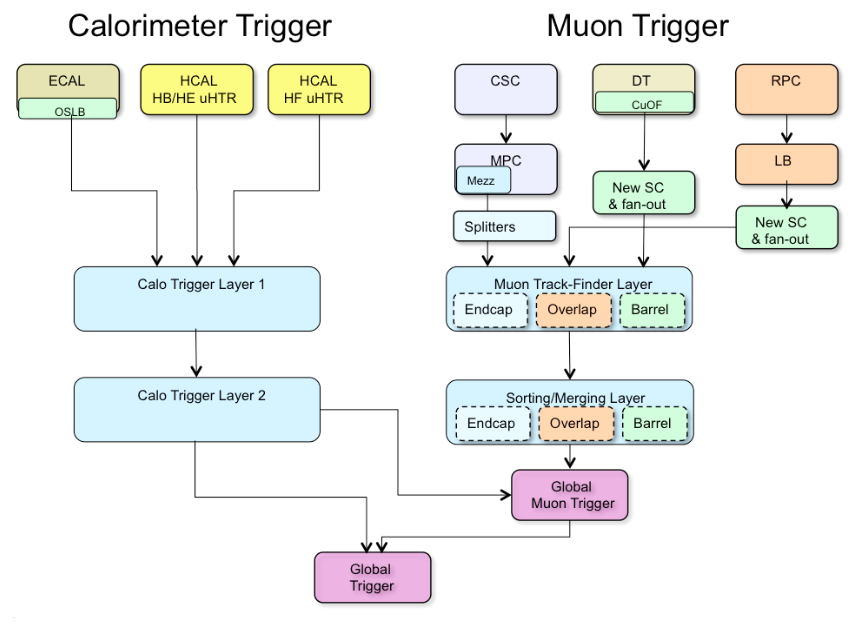
\includegraphics[width=0.8\textwidth]{img/I-3-cms/l1.png}
      \caption{Architecture of the CMS trigger system for both the calorimeter trigger and the muon trigger \cite{1748-0221-3-08-S08004}.}
      \label{fig:I-3-l1}
    \end{figure}

    The muon trigger is divided into three section: the barrel, the endcaps, and the overlap region where tracks cross both CSCs and DTs. Hits from the different chambers are combined in the Muon Track-Finder layer which uses track extrapolation and pattern recognition algorithms to create tracks. The reconstructed tracks are sent to the sorting/merging layer which selects the best candidates according to quality parameters. The best tracks are sent to the Global Muon Trigger (GMT) which uses information from the calorimeters to compute isolation values for each muon. This combined information is sent to the Global Trigger (GT) along with the data of the calorimeter. \\

    The GT implements a menu of triggers that performs selections on the reconstructed objects such as electrons, photons, or muons and take the decision to accept or reject the events. If an event is accepted, a Level-1 Accept (L1A) is issued and sent to the Trigger Control and Distribution System (TCDS) \cite{1748-0221-9-08-C08002}. The latter forwards the L1A to all the subsystems according to the readiness of the subdetectors and the data acquisition (DAQ) system. Upon reception of a L1A, the front-end electronics provides the full granularity data to the read-out DAQ which includes the HLT.

  \section{The Data Acquisition System}

    The DAQ system of CMS, shown in Figure \ref{fig:I-3-daq}, reads out the full granularity data of events from more than 650 sources in the whole detector. It is able to handle a data flow of 100 GBytes per second and redirect data to the HLT which reduces the rate of events by a factor of 1000. \\

      \begin{figure}[h!]
        \centering
        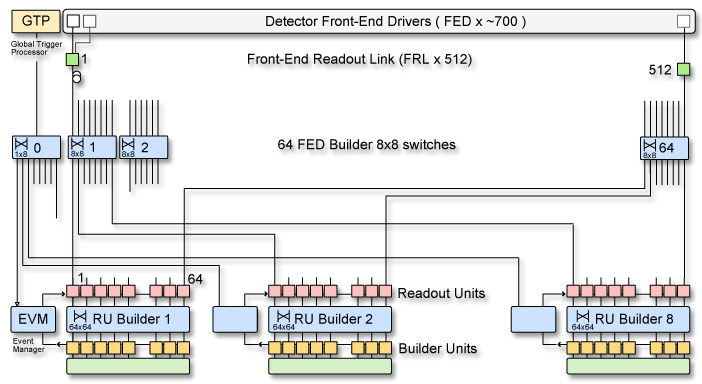
\includegraphics[width=\textwidth]{img/I-3-cms/daq.jpg}
        \caption{Architecture of the DAQ system of CMS \cite{1748-0221-3-08-S08004}.}
        \label{fig:I-3-daq}
      \end{figure}

    For each collision, the front-end electronic modules of the detectors store the full granularity data in buffers and forward reduced information to the trigger system based on which the latter will issue a L1A or not. Upon reception of an L1A from the TCDS, the Front-end drivers (FEDs) will push the full data uplink to the central DAQ system of CMS. To prevent overflow of the buffers during readout, the TCDS system provide back pressure to the FEDs. The event builder then assembles the data of the same L1A of all submodules and provides it to a single filter unit. The latter runs the HLT algorithms on the event and if accepted forwards it for storage.

    \subsection{The Event Builder}

      The event builder is composed of the FED builders and the read-out units (RU) builders. The FED builders are in charge of collecting an average size of 2 kBytes of data from the FEDs and transporting them from the underground cavern to the surface building where 72 super-fragments of roughly 16 kBytes are created. The super-fragments are distributed to the RU-builders on an event by event base, meaning that one unit will handle one event. The fragments are stored in the buffers of the RUs where the RU-builder transfers the event to the event filter.

    \subsection{The Event Filter}

      The role of the event filter is to distribute the events to worker nodes in the processing farm which run offline reconstruction algorithms to process and select events for storage. It is where the HLT is located and is in charge of reducing the 100 kHz rate of data to 100 Hz manageable by the mass storage system. Besides running reconstruction algorithms, Data Quality Monitoring (DQM) information is also generated for consistency checks. Finally, the selected events are sent for storage to data loggers.

  \section{The Upgrades of CMS}

    Following the maintenance schedule of the LHC, CMS has and will perform upgrades of its detectors to replace aging components and make use of new technologies. Due to the ambient radiation inside the cavern, the aging process of the detectors and their electronics is accelerated. Replacing these elements is thus vital in order to preserve excellent performances. Furthermore, with the increase in luminosity of the LHC, the flux of particles inside CMS will rise, yielding more difficult conditions to detect, identify, and reconstruct events. To solve this challenge, new technologies are being investigated by various collaborations within CMS.
